\documentclass[12pt,a4paper,]{book}
\def\ifdoblecara{} %% set to true
\def\ifprincipal{} %% set to true
\let\ifprincipal\undefined %% set to false
\def\ifcitapandoc{} %% set to true
\let\ifcitapandoc\undefined %% set to false
\usepackage{lmodern}
% sin fontmathfamily
\usepackage{amssymb,amsmath}
\usepackage{ifxetex,ifluatex}
%\usepackage{fixltx2e} % provides \textsubscript %PLLC
\ifnum 0\ifxetex 1\fi\ifluatex 1\fi=0 % if pdftex
  \usepackage[T1]{fontenc}
  \usepackage[utf8]{inputenc}
\else % if luatex or xelatex
  \ifxetex
    \usepackage{mathspec}
  \else
    \usepackage{fontspec}
  \fi
  \defaultfontfeatures{Ligatures=TeX,Scale=MatchLowercase}
\fi
% use upquote if available, for straight quotes in verbatim environments
\IfFileExists{upquote.sty}{\usepackage{upquote}}{}
% use microtype if available
\IfFileExists{microtype.sty}{%
\usepackage{microtype}
\UseMicrotypeSet[protrusion]{basicmath} % disable protrusion for tt fonts
}{}
\usepackage[margin = 2.5cm]{geometry}
\usepackage{hyperref}
\hypersetup{unicode=true,
            pdfauthor={Nombre Completo Autor},
              pdfborder={0 0 0},
              breaklinks=true}
\urlstyle{same}  % don't use monospace font for urls
%
\usepackage[usenames,dvipsnames]{xcolor}  %new PLLC
\IfFileExists{parskip.sty}{%
\usepackage{parskip}
}{% else
\setlength{\parindent}{0pt}
\setlength{\parskip}{6pt plus 2pt minus 1pt}
}
\setlength{\emergencystretch}{3em}  % prevent overfull lines
\providecommand{\tightlist}{%
  \setlength{\itemsep}{0pt}\setlength{\parskip}{0pt}}
\setcounter{secnumdepth}{5}
% Redefines (sub)paragraphs to behave more like sections
\ifx\paragraph\undefined\else
\let\oldparagraph\paragraph
\renewcommand{\paragraph}[1]{\oldparagraph{#1}\mbox{}}
\fi
\ifx\subparagraph\undefined\else
\let\oldsubparagraph\subparagraph
\renewcommand{\subparagraph}[1]{\oldsubparagraph{#1}\mbox{}}
\fi

%%% Use protect on footnotes to avoid problems with footnotes in titles
\let\rmarkdownfootnote\footnote%
\def\footnote{\protect\rmarkdownfootnote}


  \title{}
    \author{Nombre Completo Autor}
      \date{18/11/2021}


%%%%%%% inicio: latex_preambulo.tex PLLC


%% UTILIZA CODIFICACIÓN UTF-8
%% MODIFICARLO CONVENIENTEMENTE PARA USARLO CON OTRAS CODIFICACIONES


%\usepackage[spanish,es-nodecimaldot,es-noshorthands]{babel}
\usepackage[spanish,es-nodecimaldot,es-noshorthands,es-tabla]{babel}
% Ver: es-tabla (en: https://osl.ugr.es/CTAN/macros/latex/contrib/babel-contrib/spanish/spanish.pdf)
% es-tabla (en: https://tex.stackexchange.com/questions/80443/change-the-word-table-in-table-captions)
\usepackage[spanish, plain, datebegin,sortcompress,nocomment,
noabstract]{flexbib}
 
\usepackage{float}
\usepackage{placeins}
\usepackage{fancyhdr}
% Solucion: ! LaTeX Error: Command \counterwithout already defined.
% https://tex.stackexchange.com/questions/425600/latex-error-command-counterwithout-already-defined
\let\counterwithout\relax
\let\counterwithin\relax
\usepackage{chngcntr}
%\usepackage{microtype}  %antes en template PLLC
\usepackage[utf8]{inputenc}
\usepackage[T1]{fontenc} % Usa codificación 8-bit que tiene 256 glyphs

%\usepackage[dvipsnames]{xcolor}
%\usepackage[usenames,dvipsnames]{xcolor}  %new
\usepackage{pdfpages}
%\usepackage{natbib}




% Para portada: latex_paginatitulo_mod_ST02.tex (inicio)
\usepackage{tikz}
\usepackage{epigraph}
\input{portadas/latex_paginatitulo_mod_ST02_add.sty}
% Para portada: latex_paginatitulo_mod_ST02.tex (fin)

% Para portada: latex_paginatitulo_mod_OV01.tex (inicio)
\usepackage{cpimod}
% Para portada: latex_paginatitulo_mod_OV01.tex (fin)

% Para portada: latex_paginatitulo_mod_OV03.tex (inicio)
\usepackage{KTHEEtitlepage}
% Para portada: latex_paginatitulo_mod_OV03.tex (fin)

\renewcommand{\contentsname}{Índice}
\renewcommand{\listfigurename}{Índice de figuras}
\renewcommand{\listtablename}{Índice de tablas}
\newcommand{\bcols}{}
\newcommand{\ecols}{}
\newcommand{\bcol}[1]{\begin{minipage}{#1\linewidth}}
\newcommand{\ecol}{\end{minipage}}
\newcommand{\balertblock}[1]{\begin{alertblock}{#1}}
\newcommand{\ealertblock}{\end{alertblock}}
\newcommand{\bitemize}{\begin{itemize}}
\newcommand{\eitemize}{\end{itemize}}
\newcommand{\benumerate}{\begin{enumerate}}
\newcommand{\eenumerate}{\end{enumerate}}
\newcommand{\saltopagina}{\newpage}
\newcommand{\bcenter}{\begin{center}}
\newcommand{\ecenter}{\end{center}}
\newcommand{\beproof}{\begin{proof}} %new
\newcommand{\eeproof}{\end{proof}} %new
%De: https://texblog.org/2007/11/07/headerfooter-in-latex-with-fancyhdr/
% \fancyhead
% E: Even page
% O: Odd page
% L: Left field
% C: Center field
% R: Right field
% H: Header
% F: Footer
%\fancyhead[CO,CE]{Resultados}

%OPCION 1
% \fancyhead[LE,RO]{\slshape \rightmark}
% \fancyhead[LO,RE]{\slshape \leftmark}
% \fancyfoot[C]{\thepage}
% \renewcommand{\headrulewidth}{0.4pt}
% \renewcommand{\footrulewidth}{0pt}

%OPCION 2
% \fancyhead[LE,RO]{\slshape \rightmark}
% \fancyfoot[LO,RE]{\slshape \leftmark}
% \fancyfoot[LE,RO]{\thepage}
% \renewcommand{\headrulewidth}{0.4pt}
% \renewcommand{\footrulewidth}{0.4pt}
%%%%%%%%%%
\usepackage{calc,amsfonts}
% Elimina la cabecera de páginas impares vacías al finalizar los capítulos
\usepackage{emptypage}
\makeatletter

%\definecolor{ocre}{RGB}{25,25,243} % Define el color azul (naranja) usado para resaltar algunas salidas
\definecolor{ocre}{RGB}{0,0,0} % Define el color a negro (aparece en los teoremas

%\usepackage{calc} 


%era if(csl-refs) con dolares
% metodobib: true


\usepackage{lipsum}

%\usepackage{tikz} % Requerido para dibujar formas personalizadas

%\usepackage{amsmath,amsthm,amssymb,amsfonts}
\usepackage{amsthm}


% Boxed/framed environments
\newtheoremstyle{ocrenumbox}% % Theorem style name
{0pt}% Space above
{0pt}% Space below
{\normalfont}% % Body font
{}% Indent amount
{\small\bf\sffamily\color{ocre}}% % Theorem head font
{\;}% Punctuation after theorem head
{0.25em}% Space after theorem head
{\small\sffamily\color{ocre}\thmname{#1}\nobreakspace\thmnumber{\@ifnotempty{#1}{}\@upn{#2}}% Theorem text (e.g. Theorem 2.1)
\thmnote{\nobreakspace\the\thm@notefont\sffamily\bfseries\color{black}---\nobreakspace#3.}} % Optional theorem note
\renewcommand{\qedsymbol}{$\blacksquare$}% Optional qed square

\newtheoremstyle{blacknumex}% Theorem style name
{5pt}% Space above
{5pt}% Space below
{\normalfont}% Body font
{} % Indent amount
{\small\bf\sffamily}% Theorem head font
{\;}% Punctuation after theorem head
{0.25em}% Space after theorem head
{\small\sffamily{\tiny\ensuremath{\blacksquare}}\nobreakspace\thmname{#1}\nobreakspace\thmnumber{\@ifnotempty{#1}{}\@upn{#2}}% Theorem text (e.g. Theorem 2.1)
\thmnote{\nobreakspace\the\thm@notefont\sffamily\bfseries---\nobreakspace#3.}}% Optional theorem note

\newtheoremstyle{blacknumbox} % Theorem style name
{0pt}% Space above
{0pt}% Space below
{\normalfont}% Body font
{}% Indent amount
{\small\bf\sffamily}% Theorem head font
{\;}% Punctuation after theorem head
{0.25em}% Space after theorem head
{\small\sffamily\thmname{#1}\nobreakspace\thmnumber{\@ifnotempty{#1}{}\@upn{#2}}% Theorem text (e.g. Theorem 2.1)
\thmnote{\nobreakspace\the\thm@notefont\sffamily\bfseries---\nobreakspace#3.}}% Optional theorem note

% Non-boxed/non-framed environments
\newtheoremstyle{ocrenum}% % Theorem style name
{5pt}% Space above
{5pt}% Space below
{\normalfont}% % Body font
{}% Indent amount
{\small\bf\sffamily\color{ocre}}% % Theorem head font
{\;}% Punctuation after theorem head
{0.25em}% Space after theorem head
{\small\sffamily\color{ocre}\thmname{#1}\nobreakspace\thmnumber{\@ifnotempty{#1}{}\@upn{#2}}% Theorem text (e.g. Theorem 2.1)
\thmnote{\nobreakspace\the\thm@notefont\sffamily\bfseries\color{black}---\nobreakspace#3.}} % Optional theorem note
\renewcommand{\qedsymbol}{$\blacksquare$}% Optional qed square
\makeatother



% Define el estilo texto theorem para cada tipo definido anteriormente
\newcounter{dummy} 
\numberwithin{dummy}{section}
\theoremstyle{ocrenumbox}
\newtheorem{theoremeT}[dummy]{Teorema}  % (Pedro: Theorem)
\newtheorem{problem}{Problema}[chapter]  % (Pedro: Problem)
\newtheorem{exerciseT}{Ejercicio}[chapter] % (Pedro: Exercise)
\theoremstyle{blacknumex}
\newtheorem{exampleT}{Ejemplo}[chapter] % (Pedro: Example)
\theoremstyle{blacknumbox}
\newtheorem{vocabulary}{Vocabulario}[chapter]  % (Pedro: Vocabulary)
\newtheorem{definitionT}{Definición}[section]  % (Pedro: Definition)
\newtheorem{corollaryT}[dummy]{Corolario}  % (Pedro: Corollary)
\theoremstyle{ocrenum}
\newtheorem{proposition}[dummy]{Proposición} % (Pedro: Proposition)


\usepackage[framemethod=default]{mdframed}



\newcommand{\intoo}[2]{\mathopen{]}#1\,;#2\mathclose{[}}
\newcommand{\ud}{\mathop{\mathrm{{}d}}\mathopen{}}
\newcommand{\intff}[2]{\mathopen{[}#1\,;#2\mathclose{]}}
\newtheorem{notation}{Notation}[chapter]


\mdfdefinestyle{exampledefault}{%
rightline=true,innerleftmargin=10,innerrightmargin=10,
frametitlerule=true,frametitlerulecolor=green,
frametitlebackgroundcolor=yellow,
frametitlerulewidth=2pt}


% Theorem box
\newmdenv[skipabove=7pt,
skipbelow=7pt,
backgroundcolor=black!5,
linecolor=ocre,
innerleftmargin=5pt,
innerrightmargin=5pt,
innertopmargin=10pt,%5pt
leftmargin=0cm,
rightmargin=0cm,
innerbottommargin=5pt]{tBox}

% Exercise box	  
\newmdenv[skipabove=7pt,
skipbelow=7pt,
rightline=false,
leftline=true,
topline=false,
bottomline=false,
backgroundcolor=ocre!10,
linecolor=ocre,
innerleftmargin=5pt,
innerrightmargin=5pt,
innertopmargin=10pt,%5pt
innerbottommargin=5pt,
leftmargin=0cm,
rightmargin=0cm,
linewidth=4pt]{eBox}	

% Definition box
\newmdenv[skipabove=7pt,
skipbelow=7pt,
rightline=false,
leftline=true,
topline=false,
bottomline=false,
linecolor=ocre,
innerleftmargin=5pt,
innerrightmargin=5pt,
innertopmargin=10pt,%0pt
leftmargin=0cm,
rightmargin=0cm,
linewidth=4pt,
innerbottommargin=0pt]{dBox}	

% Corollary box
\newmdenv[skipabove=7pt,
skipbelow=7pt,
rightline=false,
leftline=true,
topline=false,
bottomline=false,
linecolor=gray,
backgroundcolor=black!5,
innerleftmargin=5pt,
innerrightmargin=5pt,
innertopmargin=10pt,%5pt
leftmargin=0cm,
rightmargin=0cm,
linewidth=4pt,
innerbottommargin=5pt]{cBox}

% Crea un entorno para cada tipo de theorem y le asigna un estilo 
% con ayuda de las cajas coloreadas anteriores
\newenvironment{theorem}{\begin{tBox}\begin{theoremeT}}{\end{theoremeT}\end{tBox}}
\newenvironment{exercise}{\begin{eBox}\begin{exerciseT}}{\hfill{\color{ocre}\tiny\ensuremath{\blacksquare}}\end{exerciseT}\end{eBox}}				  
\newenvironment{definition}{\begin{dBox}\begin{definitionT}}{\end{definitionT}\end{dBox}}	
\newenvironment{example}{\begin{exampleT}}{\hfill{\tiny\ensuremath{\blacksquare}}\end{exampleT}}		
\newenvironment{corollary}{\begin{cBox}\begin{corollaryT}}{\end{corollaryT}\end{cBox}}	

%	ENVIRONMENT remark
\newenvironment{remark}{\par\vspace{10pt}\small 
% Espacio blanco vertical sobre la nota y tamaño de fuente menor
\begin{list}{}{
\leftmargin=35pt % Indentación sobre la izquierda
\rightmargin=25pt}\item\ignorespaces % Indentación sobre la derecha
\makebox[-2.5pt]{\begin{tikzpicture}[overlay]
\node[draw=ocre!60,line width=1pt,circle,fill=ocre!25,font=\sffamily\bfseries,inner sep=2pt,outer sep=0pt] at (-15pt,0pt){\textcolor{ocre}{N}}; \end{tikzpicture}} % R naranja en un círculo (Pedro)
\advance\baselineskip -1pt}{\end{list}\vskip5pt} 
% Espaciado de línea más estrecho y espacio en blanco después del comentario


\newenvironment{solutionExe}{\par\vspace{10pt}\small 
\begin{list}{}{
\leftmargin=35pt 
\rightmargin=25pt}\item\ignorespaces 
\makebox[-2.5pt]{\begin{tikzpicture}[overlay]
\node[draw=ocre!60,line width=1pt,circle,fill=ocre!25,font=\sffamily\bfseries,inner sep=2pt,outer sep=0pt] at (-15pt,0pt){\textcolor{ocre}{S}}; \end{tikzpicture}} 
\advance\baselineskip -1pt}{\end{list}\vskip5pt} 

\newenvironment{solutionExa}{\par\vspace{10pt}\small 
\begin{list}{}{
\leftmargin=35pt 
\rightmargin=25pt}\item\ignorespaces 
\makebox[-2.5pt]{\begin{tikzpicture}[overlay]
\node[draw=ocre!60,line width=1pt,circle,fill=ocre!55,font=\sffamily\bfseries,inner sep=2pt,outer sep=0pt] at (-15pt,0pt){\textcolor{ocre}{S}}; \end{tikzpicture}} 
\advance\baselineskip -1pt}{\end{list}\vskip5pt} 

\usepackage{tcolorbox}

\usetikzlibrary{trees}

\theoremstyle{ocrenum}
\newtheorem{solutionT}[dummy]{Solución}  % (Pedro: Corollary)
\newenvironment{solution}{\begin{cBox}\begin{solutionT}}{\end{solutionT}\end{cBox}}	


\newcommand{\tcolorboxsolucion}[2]{%
\begin{tcolorbox}[colback=green!5!white,colframe=green!75!black,title=#1] 
 #2
 %\tcblower  % pone una línea discontinua
\end{tcolorbox}
}% final definición comando

\newtcbox{\mybox}[1][green]{on line,
arc=0pt,outer arc=0pt,colback=#1!10!white,colframe=#1!50!black, boxsep=0pt,left=1pt,right=1pt,top=2pt,bottom=2pt, boxrule=0pt,bottomrule=1pt,toprule=1pt}



\mdfdefinestyle{exampledefault}{%
rightline=true,innerleftmargin=10,innerrightmargin=10,
frametitlerule=true,frametitlerulecolor=green,
frametitlebackgroundcolor=yellow,
frametitlerulewidth=2pt}





\newcommand{\betheorem}{\begin{theorem}}
\newcommand{\eetheorem}{\end{theorem}}
\newcommand{\bedefinition}{\begin{definition}}
\newcommand{\eedefinition}{\end{definition}}

\newcommand{\beremark}{\begin{remark}}
\newcommand{\eeremark}{\end{remark}}
\newcommand{\beexercise}{\begin{exercise}}
\newcommand{\eeexercise}{\end{exercise}}
\newcommand{\beexample}{\begin{example}}
\newcommand{\eeexample}{\end{example}}
\newcommand{\becorollary}{\begin{corollary}}
\newcommand{\eecorollary}{\end{corollary}}


\newcommand{\besolutionExe}{\begin{solutionExe}}
\newcommand{\eesolutionExe}{\end{solutionExe}}
\newcommand{\besolutionExa}{\begin{solutionExa}}
\newcommand{\eesolutionExa}{\end{solutionExa}}


%%%%%%%%


% Caja Salida Markdown
\newmdenv[skipabove=7pt,
skipbelow=7pt,
rightline=false,
leftline=true,
topline=false,
bottomline=false,
backgroundcolor=GreenYellow!10,
linecolor=GreenYellow!80,
innerleftmargin=5pt,
innerrightmargin=5pt,
innertopmargin=10pt,%5pt
innerbottommargin=5pt,
leftmargin=0cm,
rightmargin=0cm,
linewidth=4pt]{mBox}	

%% RMarkdown
\newenvironment{markdownsal}{\begin{mBox}}{\end{mBox}}	

\newcommand{\bmarkdownsal}{\begin{markdownsal}}
\newcommand{\emarkdownsal}{\end{markdownsal}}


\usepackage{array}
\usepackage{multirow}
\usepackage{wrapfig}
\usepackage{colortbl}
\usepackage{pdflscape}
\usepackage{tabu}
\usepackage{threeparttable}
\usepackage{subfig} %new
%\usepackage{booktabs,dcolumn,rotating,thumbpdf,longtable}
\usepackage{dcolumn,rotating}  %new
\usepackage[graphicx]{realboxes} %new de: https://stackoverflow.com/questions/51633434/prevent-pagebreak-in-kableextra-landscape-table

%define el interlineado vertical
%\renewcommand{\baselinestretch}{1.5}

%define etiqueta para las Tablas o Cuadros
%\renewcommand\spanishtablename{Tabla}

%%\bibliographystyle{plain} %new no necesario


%%%%%%%%%%%% PARA USO CON biblatex
% \DefineBibliographyStrings{english}{%
%   backrefpage = {ver pag.\adddot},%
%   backrefpages = {ver pags.\adddot}%
% }

% \DefineBibliographyStrings{spanish}{%
%   backrefpage = {ver pag.\adddot},%
%   backrefpages = {ver pags.\adddot}%
% }
% 
% \DeclareFieldFormat{pagerefformat}{\mkbibparens{{\color{red}\mkbibemph{#1}}}}
% \renewbibmacro*{pageref}{%
%   \iflistundef{pageref}
%     {}
%     {\printtext[pagerefformat]{%
%        \ifnumgreater{\value{pageref}}{1}
%          {\bibstring{backrefpages}\ppspace}
%          {\bibstring{backrefpage}\ppspace}%
%        \printlist[pageref][-\value{listtotal}]{pageref}}}}
% 
%%% de kableExtra
\usepackage{booktabs}
\usepackage{longtable}
%\usepackage{array}
%\usepackage{multirow}
%\usepackage{wrapfig}
%\usepackage{float}
%\usepackage{colortbl}
%\usepackage{pdflscape}
%\usepackage{tabu}
%\usepackage{threeparttable}
\usepackage{threeparttablex}
\usepackage[normalem]{ulem}
\usepackage{makecell}
%\usepackage{xcolor}

%%%%%%% fin: latex_preambulo.tex PLLC


\begin{document}

\bibliographystyle{flexbib}



\raggedbottom

\ifdefined\ifprincipal
\else
\setlength{\parindent}{1em}
\pagestyle{fancy}
\setcounter{tocdepth}{4}
\tableofcontents

\fi

\ifdefined\ifdoblecara
\fancyhead{}{}
\fancyhead[LE,RO]{\scriptsize\rightmark}
\fancyfoot[LO,RE]{\scriptsize\slshape \leftmark}
\fancyfoot[C]{}
\fancyfoot[LE,RO]{\footnotesize\thepage}
\else
\fancyhead{}{}
\fancyhead[RO]{\scriptsize\rightmark}
\fancyfoot[LO]{\scriptsize\slshape \leftmark}
\fancyfoot[C]{}
\fancyfoot[RO]{\footnotesize\thepage}
\fi

\renewcommand{\headrulewidth}{0.4pt}
\renewcommand{\footrulewidth}{0.4pt}

\hypertarget{Seccion5}{%
\chapter{VNM-Póker y Khun-Póker}\label{Seccion5}}

En este último apartado comentaremos otro juego de azar que introdujeron
Von Newmann y Morgenstern, el VNM-Póker, junto con una variante que
amplía este juego y que se conoce como Khun-Poker. El primero fue
introducido en \emph{Theory of Games and Economic Behavior}, mientras
uqe el segundo se introdujo en \emph{A simplified two-person
poker.Contributions to the Theory of Games} .

Los dos juegos costan de dos jugadores, comunmente llamados ANN y Beth.
Cada una de ellas coge al azar una carta de la baraja sin enseñarsela a
la otra. Asi podriamos decir que los juegos presentan 4 parámetros:

\begin{enumerate}
\def\labelenumi{\arabic{enumi}.}
\item
  Hay una baraja con cartas de valores q van de 1 a \(S\).
\item
  Cada carta está representada \(r\) veces en la baraja.
\item
  Una apuesta inicial de \(m\) uds. monetarias q cada jugador realiza
  antes de empezar la partida.
\item
  Un valor final de la apuesta total de cada jugador, que denotamos como
  \(n\), al cual el jugador puede llegar añadiendo \(n-m\) uds.
  monetarias adicionales
\end{enumerate}

Como regla general se considera que \(m<n\).

\hypertarget{Seccion51}{%
\section{VNM-Póker. Explicación, estrategias y
equilibrios}\label{Seccion51}}

\textbf{\(VNM-Póker(S,r,m,n)\)} . El juego comienza repartiendo una
carta a cada jugador, y a continuación, Ann mueve primero y elige si
pasar, jugando así por m, o subir, jugando así por n.~Ahora nos
encontramos con dos posibles situaciones:

\begin{itemize}
\item
  Si Ann pasa, ambas jugadores revelan sus dos cartas, y el jugador que
  tenga la carta mas alta gana el bote, que como no se ha subido la
  apuesta es de \(2m\) uds. monetarias. Si hubiera empate, cada jugador
  recupera su dinero.
\item
  Si Ann elige subir, incrementa su apuesta hasta n.~Le toca el turno a
  Beth que tiene dos posibles movimientos, retirarse o seguir.
\end{itemize}

** Si Beth se retira, Ann se lleva el bote encima de la mesa que consta
de los \(n\) suyos mas los \(m\) de Beth, por lo que gana \(m\). La
carta de Beth no se levanta en este caso.

** Si Beth decide seguir la apuesta, ella también incrementa su apuesta
hasta \(n\). Entonces cada una revela su carta y el que tenga la carta
de mayor valor se lleva el bote completo de \(2n\) ganando así \(n\). De
la misma manera que antes, en caso de empate los jugadores recuperan su
dinero.

El juego podemos clasificarlo dentro de los de suma cero, puesto las
ganancias de uno viene de las perdidas del otro y al final el dinero que
se reparte es el dinero que proviene de las apuestas de los dos
jugadores. Procedemos ahora a representar la forma extensiva de este
juego.

\begin{figure}[H]

{\centering 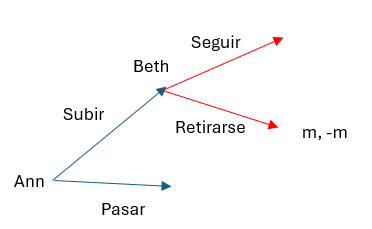
\includegraphics[width=0.8\linewidth]{extensiva_VNM} 

}

\caption{\label{forma_extensiva_VNM}VNM-Póker}\label{fig:VNM_Khun}
\end{figure}

Como hemos comentado, el juego comienza dándole una carta al azar a cada
jugador. Ann puede coger una carta cualquiera de \(1,\cdots,S\), y en
función del valor del parámetro \(r\) Beth podrá tomar también una carta
de \(1,\cdots,S\) dando \(S^2\) posibles combinaciones si \(r>1\) y en
caso de \(r = 1\), habría \(S(S-1)\) posibles combinaciones.

Con esto nos damos cuenta de que los parámetros intervienen de forma
distinta: mientras que \(m\) y \(n\) intervienen en el aspecto de
apuesta y reparto del dinero, los parámetros \(S\) y \(r\) tienen
influencia en la forma y tamaño del árbol del juego y las probabilidades
de los movimientos que dependen del azar.

Las alternativas para el movimiento aleatorio de recibir una determinada
carta no son igualmente probables. Por ejemplo, si fijamos una carta
determinada llamemosle \(C\), la probabilidad de obtener \(C\) es
\(\frac{r}{rS}= \frac{1}{S}\). una vez se saca dicha carta del mazo,
quedan \(r-1\) cartas \(C\) de un total de \(rS-1\), por lo que la
probabilidad de obtener otra carta \(C\) es \(\frac{r-1}{rS-1}\). Como
resumen:

\begin{itemize}
\tightlist
\item
  Si Ann y Beth tienen cartas de igual valor \(c\), esto tiene una
  probabilidad
\end{itemize}

\[
p_{cc}=\frac{1}{S} · \frac{r-1}{rS-1}=\frac{r-1}{S(rS-1)}
\]

\begin{itemize}
\tightlist
\item
  Si Ann y Beth tienen cartas de distinto valor \(c\) y \(d\), esto
  tiene una probabilidad
\end{itemize}

\[
p_{cd}=\frac{1}{S} · \frac{r}{rS-1}=\frac{r}{S(rS-1)}
\]

\emph{Ejemplo VNM-Póker(2,2,1,1)}

\begin{figure}[H]

{\centering 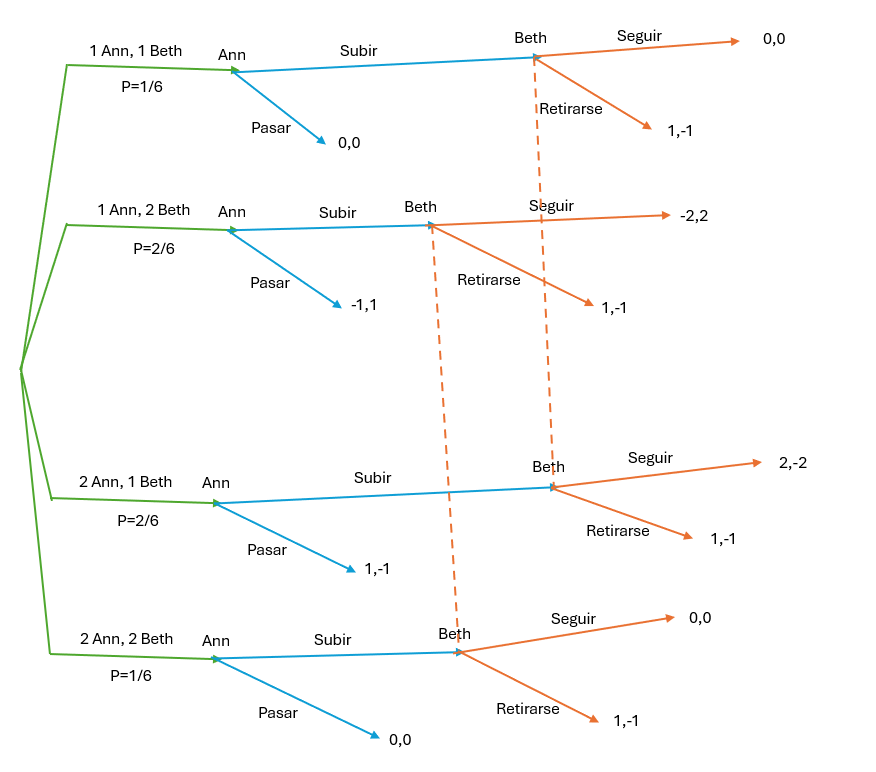
\includegraphics[width=0.8\linewidth]{Ejemplo_VNM} 

}

\caption{\label{ejemplo_VNM}VNM-Póker}\label{fig:ejemplo_VNM}
\end{figure}

\hypertarget{Seccion511}{%
\subsection{Estrategias}\label{Seccion511}}

Si \(r>1\) hay \(S*S\) diferentes combinaciones para repartir un valor a
Ann y otro a Beth. Ann como hemos dicho solo puede ver su carta por lo
que tiene \(S\) conjuntos de información. En cada uno de esos conjuntos
tiene las opciones de subir o pasar. Así pues, Ann tiene \(2^S\)
estrategias puras. Codificamos las estrategias por secuencias de \(R\) y
\(C\) (de check y raise, traducción de pasar y subir). Por ejemplo, para
\(S=4\) seria \(RCCR\) una posibilidad, que significa que Ann sube la
apuesta con las cartas mas alta y mas baja y pasa en las dos cartas
intermedias. De la misma manera, Beth tiene \(S\) conjuntos de
información con dos opciones y por lo tanto también tiene \(2^S\)
estrategias puras que están codificadas por \(C\) y \(F\) (traducciones
de seguir y retirarse).

De esta manera los posibles pagos son:

\begin{itemize}
\item
  Ann elige pasar \(\rightarrow\) \(m\), \(0\) ó \(-m\).
\item
  Ann elige subir y Beth elige retirarse \(\rightarrow\) \(m\).
\item
  Ann elige subir y Beth elige seguir \(\rightarrow\) \(n\), \(0\) ó
  \(n\).
\end{itemize}

En adelante supondremos \(S=2\) y \(r \geq 2\) . Suponiendo esto,
tenemos los siguientes conjuntos de estrategias puras para Ann es
\(\{CC \ (conservadora), CR \ (equilibrada),RC \ (inútil),RR \ (arriesgada) \}\)
y para Beth
\(\{FF \ (conservadora), FC \ (equilibrada),CF \ (inútil),CC \ (arriesgada) \}\)

Al igual que antes hicimos con la forma extensiva representamos la forma
normal del juego con \(S=2\)

\[
\begin{array}{c|c|c|c|c}
 & \text{FF} & \text{FC} & \text{CF} & \text{CC} \\
\hline
\text{CC} & 0 & 0 & 0 & 0 \\
\hline
\text{CR} & \frac{m(r-1)}{4r-2} & 0 & \frac{nr-m}{4r-2} & \frac{(n-m)r}{4r-2} \\
\hline
\text{RC} & \frac{m(3r-1)}{4r-2} & \frac{m(2r-1)-rn}{4r-2} & \frac{2mr}{4r-2} & \frac{r(m-n)}{4r-2}  \\
\hline
\text{RR} & m & \frac{m(2r-1)-rn}{4r-2} & \frac{m(2r-1)+rn}{4r-2} & 0 \\
\hline
\end{array}
\] Pasamos a comentar como hemos obtenido las expresiones para esta
tabla. Para cada par de estrategias, definimos \(u_{x,y}\) el pago que
recibe Ann cuando los jugadores siguen sus estrategias y Ann tiene una
carta de valor \(x\) y Beth una de valor \(y\), así la utilidad esperada
para Ann es la siguiente:

\[
p_{xx}u_{1,1} + p_{xy}u_{1,2} + p_{xy}u_{2,1} + p_{xx}u_{2,2}
\] donde \(p_{xx}=\frac{r-1}{4r-2}\) y \(p_{xy}=\frac{r}{4r-2}\)

Así, si Ann juega la estrategia \(RR\) y Beth juega \(FC\) tendríamos
las utilidades \(u_{1,1}=m\),\(u_{1,2}=-n\),\(u_{2,1}=m\) y\(u_{2,2}=0\)
y la utilidad que recibe Ann es:

\[
\begin{array}{ccl}
 &  & p_{xx}·m + p_{xx}·(-n) + p_{xx}·m + p_{xx}·0 \\
        & = & \frac{r-1}{4r-2}·m +\frac{r}{4r-2}·(-n) + \frac{r}{4r-2}·m +\frac{r-1}{4r-2}·0 \\
        & = & \frac{(r-1)m - rn +rm}{4r-2} \\
        & = & \frac{(2r-1)m-rn}{4r-2}·m
\end{array}
\]

Aunque hemos puesto en la tabla todas las estrategias posibles, somos
conscientes de que en algunos casos hay estrategias que están dominadas
por otras:

\begin{itemize}
\item
  Cuando Ann tiene una carta de mayor valor que Beth, subir domina a
  pasar.
\item
  Cuando Beth tiene una carta mas alta que la de Ann, seguir domina a
  retirarse.
\end{itemize}

Podemos extender esto a casos mas generales con el suiguiente teorema:

\textbf{Teorema}

Todas las estrategias de Beth, menos las de la forma \(C \cdots C\) y
las de la forma \(F \cdots FC \cdots C\) están debilmente dominadas.

Haciendo uso de este teorema podemos simplificar la forma normal del
juego a:

\[
\begin{array}{c|c|c|}
 & \text{FC} & \text{CC} \\
\hline
\text{CR} & 0  & \frac{(n-m)r}{4r-2} \\
\hline
\text{RR} & \frac{m(2r-1)-rn}{4r-2}  & 0 \\
\hline
\end{array}
\]

Una estrategia alternativa que podría seguir un jugador es la de
\emph{tirarse un farol} que consiste en, aun teniendo una carta de valor
bajo, este jugador decide subir la apuesta para intentando amedrentar al
otro jugador para así este decida retirarse. Desde el comienzo del
trabajo hemos supuesto la hipótesis de racionalidad de los jugadores por
lo que esta estrategia no tendría sentido. Pasemos ahora a analizar las
distintas estrategias.

\hypertarget{Seccion512}{%
\subsection{Análisis del juego}\label{Seccion512}}

\begin{itemize}
\tightlist
\item
  Equilibrio puro.
\end{itemize}

La entrada \(\frac{(n-m)r}{4r-2}\) siempre es \(>0\) puesto que \(n>m\).
Si \(\frac{(2r-1)m-rn}{4r-2}\) es \(<0\), la estrategia de Ann \(CR\)
domina débilmente a \(RR\), y la estrategia de Beth \(FC\) domina
débilmente a \(CC\). Por lo tanto, hay un equilibrio de Nash puro
\((CR,FC)\) con una utilidad esperada para Ann de \(0\).

\begin{itemize}
\tightlist
\item
  ¿Qué hacer si el adversario no juega de manera optima, sino mezclando
  estrategias puras no dominadas?
\end{itemize}

Vamos a suponer que el jugador que juega de esa manera es Beth, que lo
hace de esta manera: elige \(FC\) con una probabilidad \(q\) y elige
\(CC\) con probabilidad \(1-q\), es decir, elige seguir cuando tiene una
carta de valor 2 y retirarse con una probabilidad \(q\) cuando tiene una
carta de valor \(1\)

¿Qué tendría que hacer Ann en cada situación? Por un lado, si miramos
los pagos, Ann al jugar \(CR\) es \(\frac{(1-q)(n-m)r}{4r-2}\) que es
mayor o igual a \(\frac{q((2r-1)m-rn)}{4r-2}\) que es el pago al jugar
\(RR\) si (esto se da puesto que \(4r-2>0\) ya que \(r \geq 1\)):

\[
\begin{array}{rcl}
\frac{(1-q)(n-m)r}{4r-2} & \geq &\frac{q((2r-1)m-rn)}{4r-2}\\
(1-q)(n-m)r & \geq & q((2r-1)m-rn) \\
(n-m)r -q(n-m)r & \geq & q((2r-1)m-rn)\\
(n-m)r & \geq & q[((2r-1)m-rn)+(n-m)r]\\
(n-m)r & \geq & q[(r-1)m]\\
\end{array}
\]

Como \(r \geq 2\) tenemos que \((r-1)m >0\), lo podemos pasar dividiendo
sin cambiar el signo de la desigualdad y tendríamos:

\[
q^* = \frac{(n-m)r}{(r-1)m} \geq q
\] Por lo que Ann debe jugar \(CR\) si Beth juega \(FC\), mientras que
en otro caso Ann debería jugar \(RR\), jugando así de manera opuesta al
comportamiento de Beth. Por su parte, Beth debería copiar las jugadas
que haga Ann.

\begin{itemize}
\tightlist
\item
  Equilibrio mixto.
\end{itemize}

Si \(\frac{n}{m} \geq 2- \frac{1}{2}\) no hay equilibrio de Nash puro y
tendríamos q encontrar uno mixto.

Supongamos que Ann juega \(CR\) con probabilidad \(p\) y \(RR\) con
probabilidad \(1-p\), y Beth juega \(FC\) con probabilidad \(q\) y
\(CC\) con probabilidad \(1-q\). Cada una de las estrategias puras
\((CR,FC)\) y \((RR,CC)\) es una mejor respuesta a ellas y concluimos
con:

\[
p=\frac{(2r-1)m-rn}{(r-1)m} \ y \ q=\frac{(n-m)r}{(r-1)m}
\]

\hypertarget{Seccion52}{%
\section{Khun-Póker. Cambios respecto al VNM-Póker}\label{Seccion52}}

\textbf{\(Kuhn-Poker(S,r,m,n)\)} Este juego extiende el VNM-Póker. Si
Ann decide pasar los jugadores juegan un VNM-Póker con los roles
cambiados. Ann mueve primero eligiendo entre pasar o subir.

\begin{itemize}
\tightlist
\item
  Si Ann decide pasar, entonces Beth puede pasar o subir:
\end{itemize}

** Si Beth pasa, ambas cartas se levantan para ser visibles y el que
tenga la carta mas alta se lleva el bote, mientras que si empatan los
jugadores recuperan su dinero.

** Si Beth elige subir, incrementa su apuesta hasta \(n\). Entonces Ann
tiene dos opciones, retirarse o seguir.

*** Si Ann se retira, Beth se lleva la cantidad de \(n+m\), y la carta
de Ann no se revela.

*** Si Ann sigue, incrementa su apuesta hasta \(n\). Entonces ambas
cartas se revelan y el que tenga la carta mas alta se lleva los \(2n\)
de la apuesta y recuperan su dinero en caso de empate.

\begin{itemize}
\tightlist
\item
  Si Ann sube, el juego funciona como el VNM-Póker cuando Ann sube.
\end{itemize}

\begin{figure}[H]

{\centering 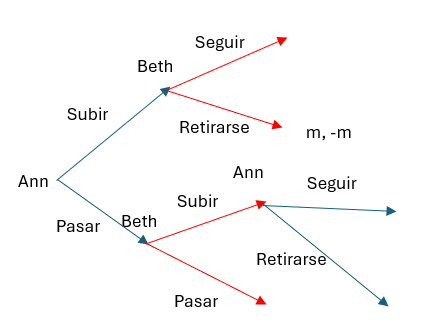
\includegraphics[width=0.8\linewidth]{extensiva_Kuhn} 

}

\caption{\label{forma_extensiva_VNM}Kuhn-Póker}\label{fig:forma_extensiva_VNM}
\end{figure}

\hypertarget{Seccion521}{%
\subsection{Estrategia}\label{Seccion521}}

Ann tiene \(2S\) conjuntos de información: o bien ella hace su primer
movimiento, subir o pasar, o Ann ha pasado en su primer movimiento, Beth
ha subido y entonces Ann puede seguir o retirarse. En todos eso casos,
ella solo conoce el valor de su carta. Beth tiene \(2S\) conjuntos de
información, determinados por el valor de su carta y en función de si
Ann ha subido o pasado, con \(S\) conjuntos de información en cada uno.

Por lo tanto, Ann tiene \(2^{2S}\) estrategias puras, indicadas por
\(S\) letras que pueden ser como en la sección \(\ref{Seccion511}\)
\(R\) o \(C\) para las elecciones de subir o pasar, y también \(S\)
letras \(F\) o \(C\) para la elección de retirarse o seguir. Así, para
\(S=2\) tenemos 16 estrategias puras, que son \(CCFF\), \(CCFC\),
\(CCCF\), \(CCCC\), \(CRFF\), \(CRFR\), \(CRCF\), \(CRCC\), \(RCFF\),
\(RCFC\), \(RCCF\), \(RCCC\), \(RRFF\),\(RRFC\), \(RRCF\), y \(RRCC\).

De la misma manera, Beth también tiene \(2S\) conjuntos de información,
\(S\) cuando Ann sube y otros \(S\) cuando Ann pasa, así para \(S=2\)
tendríamos: \(FFCC\), \(FFCR\), \(FFRC\), \(FFRR\), \(FCCC\), \(FCCR\),
\(FCRC\), \(FCRR\), \(CFCC\), \(CFCR\), \(CFRC\), \(CFRR\),
\(CCCC\),\(CCCR\), \(CCRC\), y \(CCRR\).

Hemos podido eliminar algunas estrategias por estar dominadas al igual
que antes. Si Ann tiene un valor de carta mayor que el de Beth, y ella
pasa cuando Beth sube, siempre es mejor para Ann seguir y no retirarse
puesto que retirándose pierde \(m\) uds. monetarias mientras que si
sigue no puede perder. Si Ann tiene un valor de carta mas alto, subir no
domina necesariamente a pasar, ya que depende de la estrategia de Beth.
Si Beth tiene una carta de valor mas alto que Ann, seguir domina a
retirarse y subir domina a pasar.

\bibliography{bib/library.bib,bib/paquetes.bib}


%


\end{document}
